\documentclass[border=4pt]{standalone}
\usepackage{tikz}
\usetikzlibrary{positioning, arrows.meta, shapes.geometric, calc, fit, backgrounds}
\usepackage{amsmath,amssymb}

\begin{document}
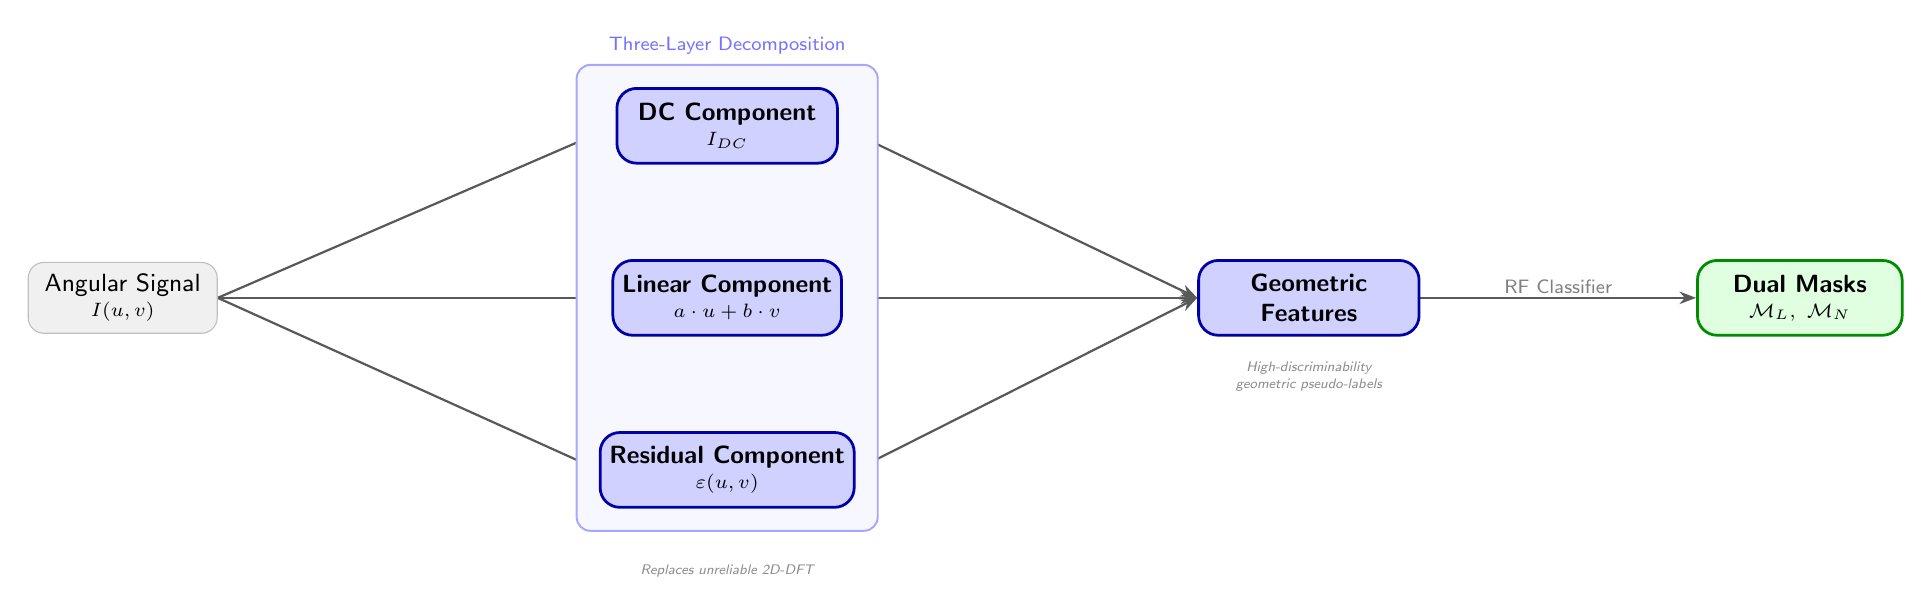
\begin{tikzpicture}[
  input/.style={draw, rounded corners=2mm, minimum width=2.4cm, minimum height=0.9cm,
                fill=gray!12, draw=gray!50, align=center, font=\sffamily\small},
  innov/.style={draw, rounded corners=2.5mm, minimum width=2.8cm, minimum height=0.95cm,
                fill=blue!18, draw=blue!65!black, line width=1pt, align=center,
                font=\sffamily\small\bfseries},
  output/.style={draw, rounded corners=2.5mm, minimum width=2.6cm, minimum height=0.95cm,
                 fill=green!12, draw=green!55!black, line width=1pt, align=center,
                 font=\sffamily\small\bfseries},
  arr/.style={-{Stealth[length=6pt]}, thick, color=black!65},
  lbl/.style={font=\sffamily\scriptsize, text=black!50, fill=white, inner sep=1pt},
  gbox/.style={draw=blue!35, rounded corners=5pt, inner sep=8pt, line width=0.7pt, fill=blue!3},
  note/.style={font=\sffamily\tiny\itshape, text=black!45, align=center},
]

% === Nodes ===

% Input
\node[input] (m1) {Angular Signal\\[-2pt]{\scriptsize $I(u,v)$}};

% Three-layer decomposition
\node[innov, right=5cm of m1] (m3) {Linear Component\\[-2pt]{\scriptsize $a \cdot u + b \cdot v$}};
\node[innov, above=1.2cm of m3] (m2) {DC Component\\[-2pt]{\scriptsize $I_{DC}$}};
\node[innov, below=1.2cm of m3] (m4) {Residual Component\\[-2pt]{\scriptsize $\varepsilon(u,v)$}};

% Geometric Features
\node[innov, right=4.5cm of m3] (m5) {Geometric\\Features};

% Dual Masks
\node[output, right=3.5cm of m5] (m6) {Dual Masks\\[-2pt]{\scriptsize $\mathcal{M}_L,\ \mathcal{M}_N$}};

% === Arrows on background layer ===
\begin{scope}[on background layer]
  % Fan-out from m1 to decomposition
  \draw[arr] (m1.east) -- (m2.west);
  \draw[arr] (m1.east) -- (m3.west);
  \draw[arr] (m1.east) -- (m4.west);

  % Convergence from decomposition to m5
  \draw[arr] (m2.east) -- (m5.west);
  \draw[arr] (m3.east) -- (m5.west);
  \draw[arr] (m4.east) -- (m5.west);

  % m5 to m6 with RF Classifier label
  \draw[arr] (m5) -- node[above, lbl] {RF Classifier} (m6);
\end{scope}

% === Grouping box around decomposition ===
\begin{scope}[on background layer]
  \node[gbox, fit=(m2)(m3)(m4),
        label={[font=\sffamily\scriptsize, text=blue!55]above:Three-Layer Decomposition}] (g1) {};
\end{scope}

% === Annotations ===
\node[note, below=0.3cm of g1] {Replaces unreliable 2D-DFT};
\node[note, below=0.2cm of m5] {High-discriminability\\geometric pseudo-labels};

\end{tikzpicture}
\end{document}